\documentclass[border=5pt]{standalone}
\usepackage[defaultfam,tabular,lining]{montserrat}
\usepackage[T1]{fontenc}
\renewcommand{\familydefault}{\sfdefault}
\usepackage{amsmath}
\usepackage[eulergreek]{sansmath}
\sansmath
\usepackage{tikz}
\usetikzlibrary{arrows.meta, positioning, calc, fit, backgrounds}
\usepackage{fontawesome5}

% Palette (matching fl-comparison.tex)
\definecolor{inkblack}{HTML}{111111}
\definecolor{pbpurple}{HTML}{6D28D9}
\definecolor{pbpurplefill}{HTML}{F5F3FF}
\definecolor{devicegrey}{HTML}{94A3B8}
\definecolor{devicefill}{HTML}{E2E8F0}
\definecolor{trustteal}{HTML}{0D9488}
\definecolor{dimgrey}{HTML}{C4B5FD}
\definecolor{panelbg}{HTML}{F9FAFB}
\definecolor{panelborder}{HTML}{E5E7EB}

\newcommand{\treeicon}[3]{%
  \begin{scope}[shift={(#1,#2)}, scale=0.4]
    \fill[#3] (0,0) circle (3pt);
    \fill[#3] (-0.7,-0.55) circle (3pt);
    \fill[#3] (0.7,-0.55) circle (3pt);
    \fill[#3] (-1.05,-1.1) circle (2.5pt);
    \fill[#3] (-0.35,-1.1) circle (2.5pt);
    \fill[#3] (0.35,-1.1) circle (2.5pt);
    \fill[#3] (1.05,-1.1) circle (2.5pt);
    \draw[#3, line width=0.6pt] (0,0) -- (-0.7,-0.55);
    \draw[#3, line width=0.6pt] (0,0) -- (0.7,-0.55);
    \draw[#3, line width=0.5pt] (-0.7,-0.55) -- (-1.05,-1.1);
    \draw[#3, line width=0.5pt] (-0.7,-0.55) -- (-0.35,-1.1);
    \draw[#3, line width=0.5pt] (0.7,-0.55) -- (0.35,-1.1);
    \draw[#3, line width=0.5pt] (0.7,-0.55) -- (1.05,-1.1);
  \end{scope}%
}

% Phone icon command
\newcommand{\phoneicon}[2]{%
  \draw[devicegrey, fill=devicefill, rounded corners=1.5pt, line width=0.5pt]
    (#1, #2) rectangle ++(0.3, 0.44);
  \draw[devicegrey, fill=devicegrey, line width=0.3pt, rounded corners=0.5pt]
    (#1+0.05, #2+0.36) rectangle ++(0.2, 0.04);
}

\begin{document}
\begin{tikzpicture}[
    font=\footnotesize,
    cbox/.style 2 args={draw=#1, fill=#2, rounded corners=3pt, minimum height=1.5cm,
                        text width=2.2cm, align=center, line width=1.2pt, text=inkblack},
    shB/.style={cbox={pbpurple}{pbpurplefill}},
    aggB/.style={cbox={pbpurple}{pbpurplefill}},
    mbox/.style={draw=inkblack, fill=white, rounded corners=3pt,
                 minimum height=1.1cm, minimum width=1.4cm, align=center,
                 line width=1pt},
    panel/.style={draw=panelborder, fill=panelbg, rounded corners=4pt,
                  line width=0.8pt, text=inkblack, align=left,
                  text width=7.5cm, inner sep=10pt},
    arr/.style={-{Stealth[length=5pt,width=3.5pt]}, line width=1.1pt, pbpurple},
    arrdim/.style={-{Stealth[length=5pt,width=3.5pt]}, line width=1.1pt, dimgrey, densely dashed},
    ret/.style={-{Stealth[length=5pt,width=3.5pt]}, line width=1.1pt, pbpurple, densely dashed},
    lbl/.style={font=\scriptsize\bfseries, text=inkblack, inner sep=2pt},
  ]

  % ===== TIER 1: CLIENTS (top) =====
  % Client devices with trust boundaries
  \foreach \i/\lbl in {0/C$_1$, 1/C$_2$, 2/C$_3$, 4/C$_n$} {
    \pgfmathsetmacro{\xx}{1.5 + \i*1.5}
    % Trust boundary (teal dashed)
    \draw[trustteal, densely dashed, line width=0.7pt, rounded corners=3pt]
      (\xx-0.1, 8.0) rectangle ++(0.5, 0.7);
    % Phone icon
    \phoneicon{\xx}{8.1}
    % Label to the left of phone
    \node[font=\tiny\bfseries, text=pbpurple, anchor=east] at (\xx-0.15, 8.32) {\lbl};
  }
  % Ellipsis between C3 and Cn
  \node[font=\footnotesize, text=devicegrey] at (6.15, 8.35) {$\cdots$};

  % Tier label above clients
  \node[font=\scriptsize\bfseries, text=inkblack] at (4.5, 8.95) {Clients ($N$ total, 1 sample each)};

  % Trust boundary label — below client labels
  \node[font=\tiny\bfseries, text=trustteal] at (4.5, 7.6) {trust boundary = each device};

  % ===== ARROWS: Clients -> Shareholders =====
  % Fan-out from C1 to all shareholders
  \draw[arr] (1.65, 8.0) -- (1.8, 6.0);
  \draw[arr] (1.65, 8.0) -- (4.5, 6.0);
  \draw[arrdim] (1.65, 8.0) -- (7.2, 6.0);

  \node[lbl] at (0.6, 7.1) {secret shares};
  \node[font=\tiny\bfseries, text=inkblack] at (0.6, 6.8) {(\textcolor{pbpurple}{features} / \textcolor{pbpurple}{gradients})};

  % ===== TIER 2: SHAREHOLDERS (middle) =====
  \node[shB] (sh1) at (1.8, 5.05) {{\normalsize\faHospital}\\[-1pt]\textbf{Shareholder 1}\\[-2pt]{\tiny\itshape e.g.\ Hospital}};
  \node[shB] (sh2) at (4.5, 5.05) {{\normalsize\faCloud}\\[-1pt]\textbf{Shareholder 2}\\[-2pt]{\tiny\itshape e.g.\ Cloud}};
  \node[shB, draw=dimgrey, text=devicegrey, fill=white] (sh3) at (7.2, 5.05) {{\normalsize\faLandmark}\\[-1pt]\textbf{Shareholder 3}\\[-2pt]{\tiny\itshape e.g.\ Regulator}};

  % ===== TIER 3: AGGREGATOR =====
  \node[aggB, text width=2.8cm] (agg) at (4.5, 2.0)
    {{\normalsize\faServer}\\[-1pt]\textbf{Aggregator}};

  % ===== ARROWS: Shareholders -> Aggregator =====
  \draw[arr] (sh1.south) -- ([xshift=-10pt]agg.north);
  \draw[arr] (sh2.south) -- (agg.north);
  \draw[arrdim] (sh3.south) -- ([xshift=10pt]agg.north);

  \node[lbl, anchor=east] at (1.3, 3.5) {partial sums};

  % Threshold annotation
  \node[font=\tiny\bfseries\itshape, text=inkblack, anchor=west, align=left] at (6.5, 3.5)
    {threshold reconstruction\\($m$-of-$k$)};

  % Model
  \node[mbox] (model) at (4.5, 0.2) {};
  \treeicon{4.5}{0.45}{inkblack}
  \node[font=\tiny\bfseries, text=inkblack] at (4.5, -0.15) {Model};

  % Arrow: aggregator -> model
  \draw[arr] (agg.south) -- (model.north);

  % ===== RETURN ARROW =====
  \draw[ret] (model.east) -- (9.0, 0.2) -- (9.0, 8.35) -- (7.9, 8.35);
  \node[lbl, anchor=east] at (8.8, 7.1) {bin edges,};
  \node[lbl, anchor=east] at (8.8, 6.8) {split decisions};

  % ===== PHASE PANELS (right side) =====
  % Phase 1
  \node[panel, anchor=north west] (p1) at (10.5, 9.5) {
    {\normalsize\bfseries Phase 1: Statistics}\\[4pt]
    Clients share $x_i$, $x_i^2$\\[2pt]
    Aggregator computes:\\[2pt]
    \quad $\mu = \dfrac{\textcolor{pbpurple}{\boldsymbol{\sum} x}}{N}$, \quad $\sigma^2 = \dfrac{\textcolor{pbpurple}{\boldsymbol{\sum} x^2}}{N} - \mu^2$\\[6pt]
    Bins: $B\!+\!2$ edges at equal-probability\\quantiles of $\mathcal{N}(\mu, \sigma^2)$
  };

  % Phase 2
  \node[panel, anchor=north west] (p2) at (10.5, 5.9) {
    {\normalsize\bfseries Phase 2: Gradients}\\[4pt]
    Clients share $g_i$, $h_i$ per bin\\[2pt]
    Per bin $b$: $G_b = \textcolor{pbpurple}{\boldsymbol{\sum} g_i}$, \; $H_b = \textcolor{pbpurple}{\boldsymbol{\sum} h_i}$\\[4pt]
    Best split: $\max_b \;\dfrac{G_b^{\,2}}{H_b + \lambda}$
  };

  % Privacy
  \node[panel, anchor=north west] (p3) at (10.5, 3.0) {
    {\normalsize\bfseries Privacy Guarantees}\\[4pt]
    \textbullet{} Shareholders see random shares\\[1pt]
    \textbullet{} Aggregator sees only sums\\[1pt]
    \textbullet{} No individual values revealed\\[5pt]
    All computations use only \textcolor{pbpurple}{\textbf{sums}} of\\secret-shared values
  };

  % ===== LEGEND (top right, above panels, in its own box) =====
  \node[panel, anchor=north west, text width=7.5cm, inner sep=8pt] at (10.5, 10.3) {
    {\small $\mathbf{x}$ = feature value \quad $\mathbf{g}$ = gradient \quad $\mathbf{h}$ = hessian}
  };

\end{tikzpicture}
\end{document}
